\documentclass{article}
\usepackage[utf8]{inputenc}
\usepackage{scrextend}
\usepackage[acronym]{glossaries}
\usepackage{tasks}
\usepackage{graphicx}
\usepackage{amssymb}
\addtokomafont{labelinglabel}{\sffamily}
\textwidth = 470pt
\marginparwidth = 0pt
\oddsidemargin = 0pt

\makeglossaries
% abbreviations:
\newacronym{cbs}{CBS}{Central Bureau of Statistics}
\newacronym{gps}{GPS}{Global Positioning System}
\newacronym{gdpr}{GDPR}{General Data Protection Regulation}

\title{Social Physics On Instagram Key Concepts}
\author{
  Hendriks, Jandie\\
  \and
  Witlox, Timothy\\
  \and
  Kooijman, Jeroen\\
  \and
  Weijs, Thomas\\
  \and
  Theunissen, Ties\\
  \and
  Melskens, Demian\\
}
\date{November 2018}

\begin{document}
\maketitle
\pagenumbering{gobble}
\pagebreak
\tableofcontents
\pagebreak
\pagenumbering{arabic}
\section{Introduction}
\subsection{Professional Task}
This document serves as a research paper for the social physics course. The goal is to take a closer look at human behaviour within the scope of our professional task. The aforementioned professional task consists of an analysis of the social media service Instagram for the \gls{cbs}. Using a data-set with information about public posts (\gls{gps}, likes, hashtags, etc.) we try to answer two questions within the professional task. Human behaviour plays an important role in answering these questions. 
\begin{enumerate}
	\item \textit{Can we sort the posts into defined categories using machine learning?}
	\item \textit{What information can be gathered based on the given \gls{gps} data?}
\end{enumerate}
\subsection{Goal}
Within the broad subject that is social physics, there are some key concepts we want to take a look at in this document. Furthermore we'll set up a mind-map visualizing where these key concepts influence our professional task. 

\pagebreak

\section{Key Concepts}
\subsection{Idea Flow}
The flow of ideas is the way information spreads through social networks. In the modern day, the manner of spreading is mostly digital. Think of the common social media networks like Facebook, Twitter and Instagram. More idea focused networks like "TED: Ideas Worth Spreading" and forum sites like Reddit also play an important role in the sharing of information. Idea flow in real life still happens too, and for good reason. Knowledge sharing sessions play an important role within companies and schools. These are purely designed to share ideas by discussing problems and solutions. ``Idea flow is the propagation of behaviors and beliefs through social networks by means of social learning and social pressure." -Alex Pentland.

We all make use of the stream of ideas, ideas that are the examples and stories of the people who surround us. Exposure to this stream shapes our habits and beliefs. The idea flow within these streams binds us together into a sort of collective intelligence, one based on shared learning. In the connected world we live in, the most important decision is who to follow. One measure to use when evaluating a possible following is idea flow: how many innovative ideas is the target generating, and what proportion of those do other creative people find intriguing? These considerations are what makes it so that start-up companies often hire creative and "out-of-the-box" people.

\subsection{Social Learning}
Social learning is a theory of learning and social behaviour that explains that we can acquire new behaviours by observing and imitating others. This is where the metaphor ``monkey see, monkey do'' comes from. People can learn by looking at others and seeing what the result is of their actions. This way people are able to adapt and learn very fast. On the contrary, this can also work against us, for example with cyber bullying. Akers and Burgess (criminologists) hypothesized that observed or experienced positive rewards and lack of punishment for aggressive behaviors reinforces aggression. In this way, social learning can influence us in both positive and negative ways.

\subsection{Living laboratories}
A living lab is a research concept. This concept is based on a systematic user co-creation approach integrating research and innovation processes. These processes are integrated through the experimentation and evaluation of innovative ideas. Such use cases involve user groups as observed subjects. This approach allows all involved stakeholders to consider both the global performance of a product and its potential adoption by users. This may be used at the earlier stage of research and development but is useful through all elements of the product life-cycle. The living lab process is based on the following four main activities:
\begin{enumerate}
    \item Co-creation: contains methods like crowd-sourcing and crowd-casting to bring together a diversity of views, constraints and knowledge sharing to encourage the creation of new scenarios and concepts.
    \item Exploration: engage all stakeholders, especially user communities, at the earlier stage of the co-creation process for discovering emerging scenarios, usages and behaviours through live scenarios in real or virtual environments (e.g. virtual reality, augmented reality, mixed reality).
    \item Experimentation: implement experimental versions to experience scenarios with a large number of users while collecting data which will be analyzed in their context during the activity.
    \item Evaluation: evaluate new ideas and innovative concepts on their usefulness to see the real life situations on various aspects. Make observations on the potentiality of a viral adoption of new concepts through a confrontation with users' experiences.
\end{enumerate}

\subsection{Reality Mining}
Reality mining is the collection and analysis of machine-gathered environmental data. This includes data that is used and sent in the background by a wireless machine such as a mobile phones and \gls{gps} systems to gather what people do, where they go, and with whom they communicate. This way you will get more accurate data rather than looking at subjective data someone has posted on his/her account. This is something that is used by most big companies to get to know more about their customers, even to an extend where people were concerned for their privacy. This is also why the \gls{gdpr} was created. This data that is gathered through reality mining is used in big data projects to analyze and visualize customer behaviour. This is then used to find new strategies and get an insight in the consumers of the product or service.

\subsection{Fast Thinking, Slow Thinking and Free Will}
\subsubsection{Fast and Slow Thinking}
The brain and mind consists of two sides. First, let's have a look at the brain side. The left side of the brain is responsible for controlling the right side of the body. It also performs tasks that have to do with logic, such as in science and mathematics. On the other hand, the right hemisphere coordinates the left side of the body, and performs tasks that have do with creativity and the arts. Now there is also a theory that the mind consists out of two parts:
\begin{itemize}
    \item \textbf{System 1:} Fast, automatic, frequent, emotional, stereotypical, unconscious.
    \item \textbf{System 2:} Slow, infrequent, logical, calculating, conscious, with effort.
\end{itemize}
To illustrate both of these systems it is best to look at some examples. let's start with system 1, which is the automatic and emotional side. Seeing that an object is further away than another object is instant and fast. Another example is driving a car (for someone who can drive) on an empty road. It is often said that this creates a blackout effect where people can't remember is because the automatic part of the brain (system 1) took over.

Next up are some examples of system 2, the calculating and conscious side. Finding a women with gray hair in a crowd for instance, is something you'd consciously have to look for and requires effort. Counting the number of occurrences of a specific letter in a text is also a calculating and slow action which is fulfilled by system 2.
\subsubsection{Free Will}
Free will is shortly said the ability to choose between different possible courses of action based on nothing but you as a person. Some conceive free will to be the capacity to make choices in which the outcome has not been determined by past events. This would suggest that if only one course of events is possible, this would be inconsistent with the existence of free will. This problem has been identified in ancient Greek philosophy and remains a major focus of philosophical debate. There are multiple different views on this concept ranging from absolute free will to no free will.

Within our professional task the views on free will are split 50-50. Half of are group are under the impression that free will is a myth as everything influences our decision making, and that the feeling of free will is based upon your environment and how you were raised. The other half thinks that there is at least some form of free will in the decisions that we make in the everyday life. Especially the small and impulsive decisions would be made independently from influences.

\section{Mind-map}
    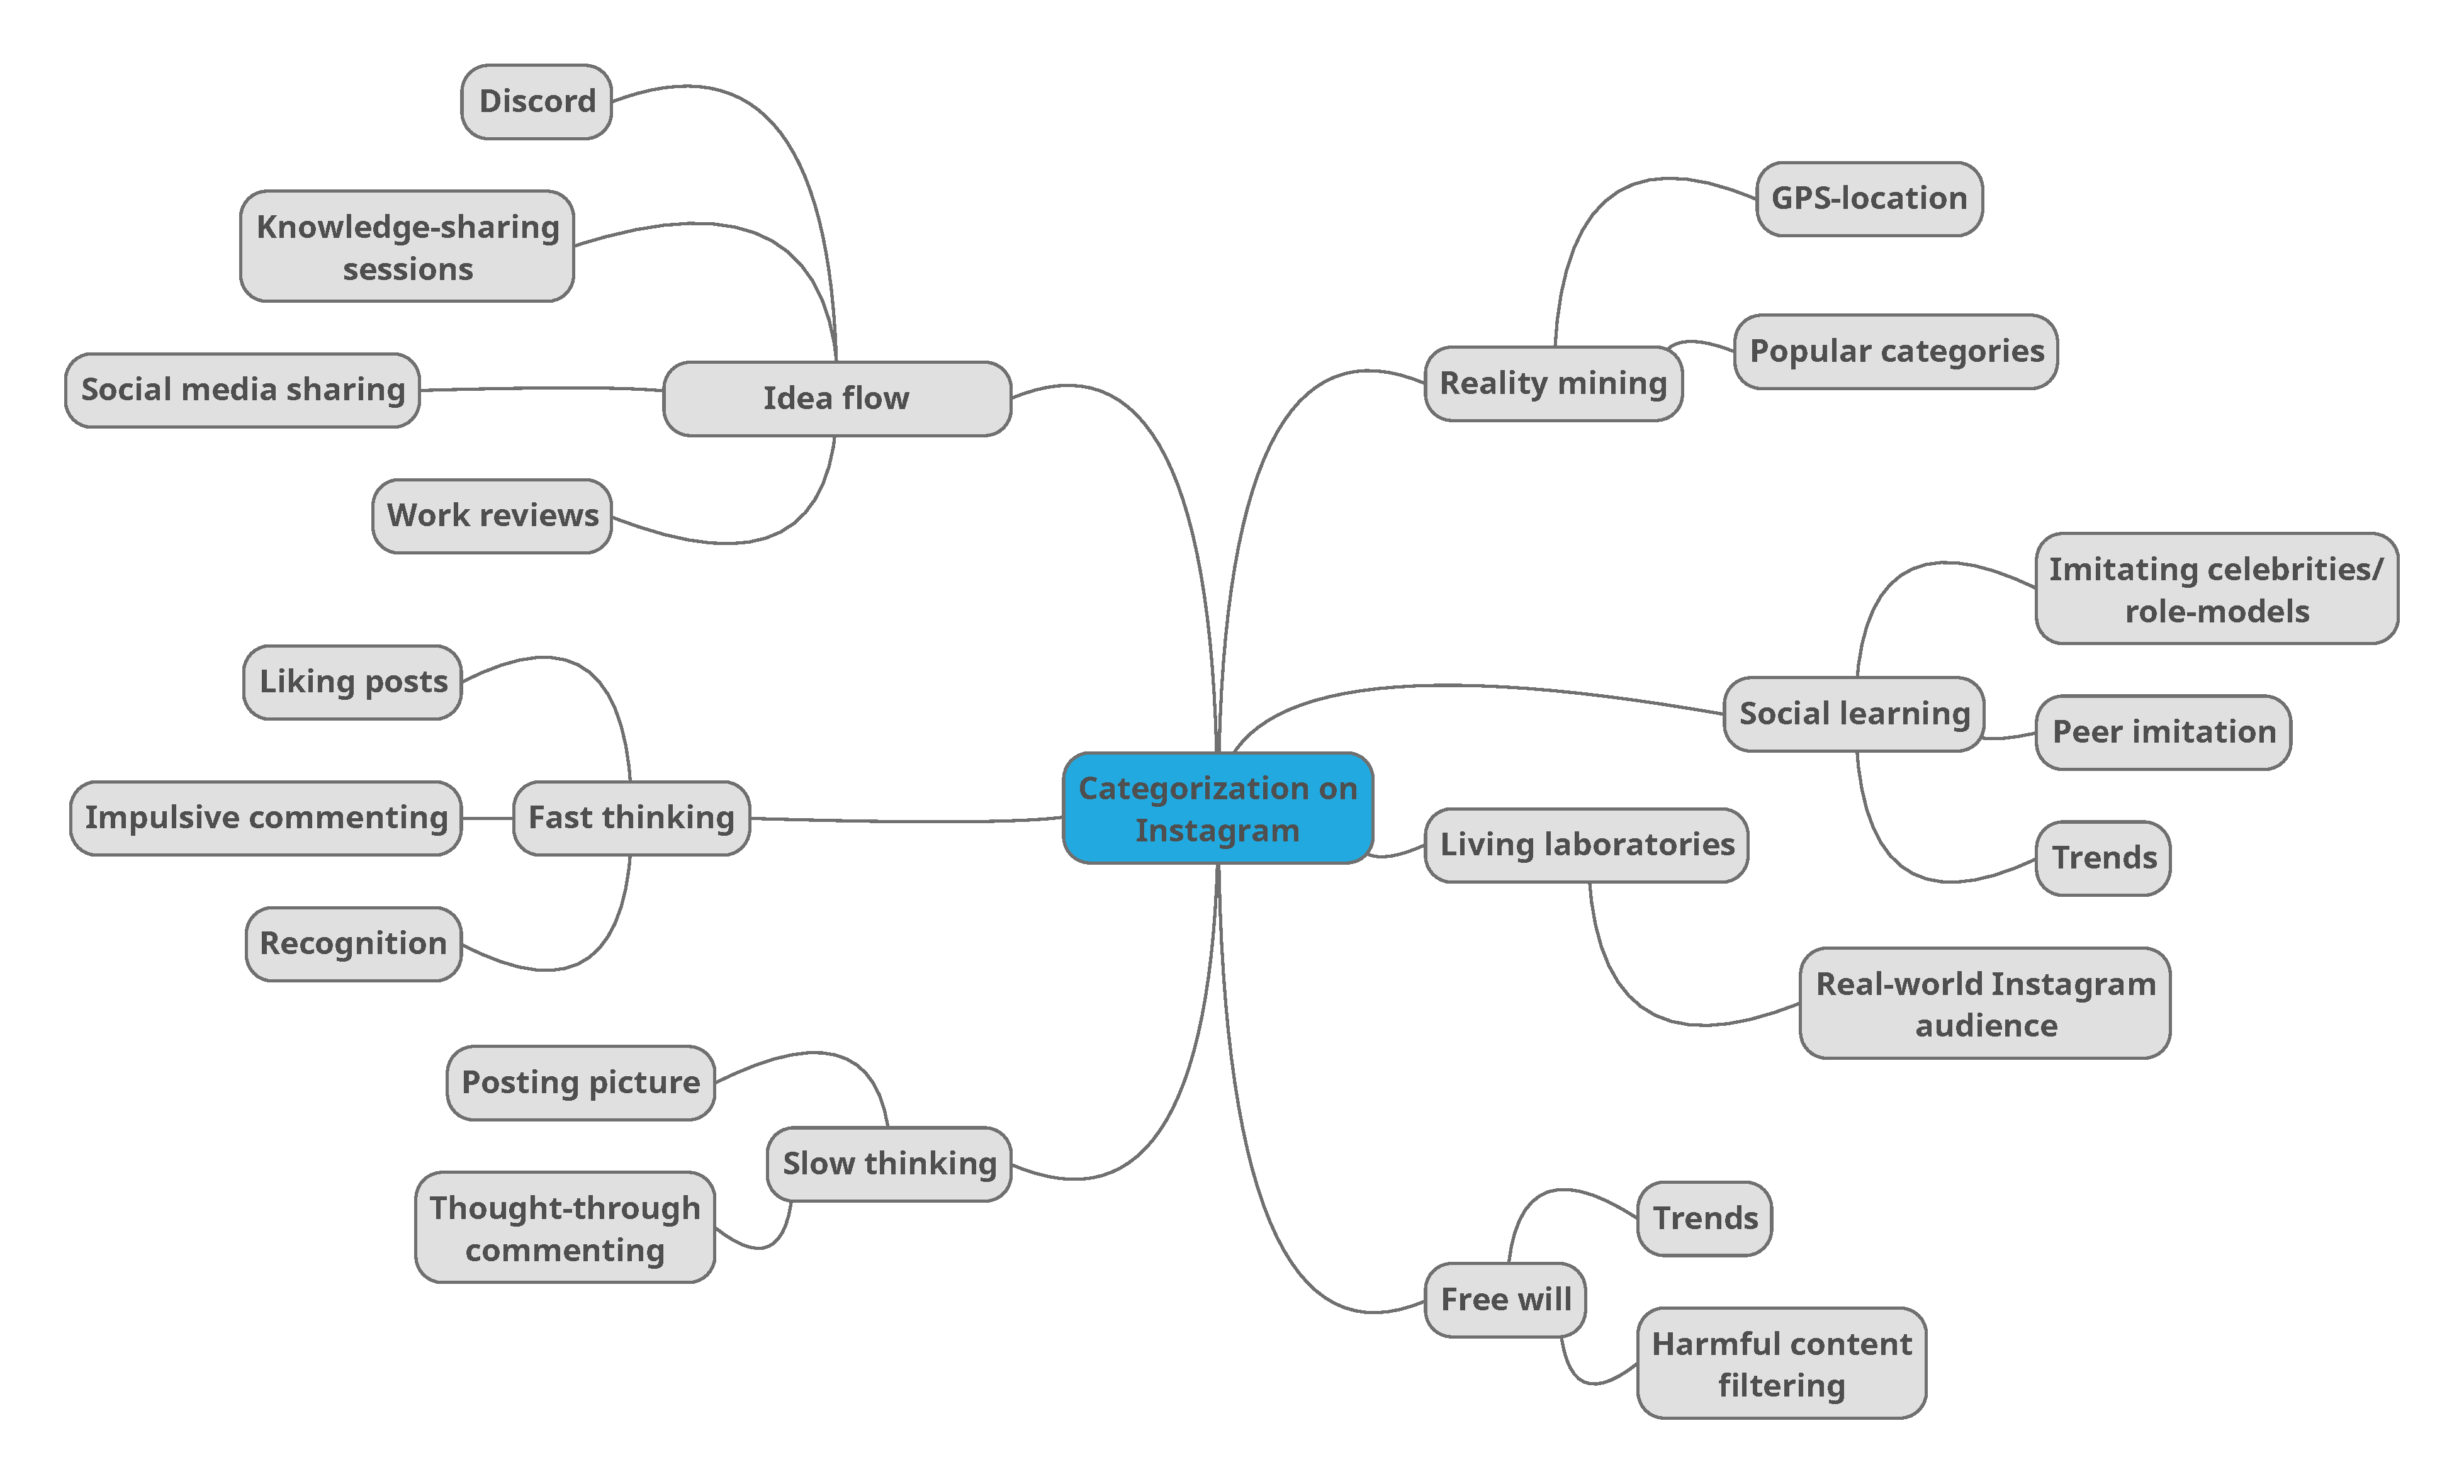
\includegraphics[width=15cm,height=15cm,keepaspectratio]{mindmap.pdf}
    ldjejd djaf 

\pagebreak
\printglossary[type=\acronymtype,title=\section{Abbreviations}]

\end{document}